\section{Simulation Analysis and Comparison with Theoretical Results}
\label{sec:simulation}

\subsection{Transient Analysis}


Figure~\ref{fig:trans2} shows the simulated transient analysis results for input voltage of the secondary circuit,
the envelope detector output voltage, $V_3$, the voltage regulator output voltage, $V_4$ 
and the average voltage difference, $V_4$-12 Volts.

\begin{figure}[H] \centering
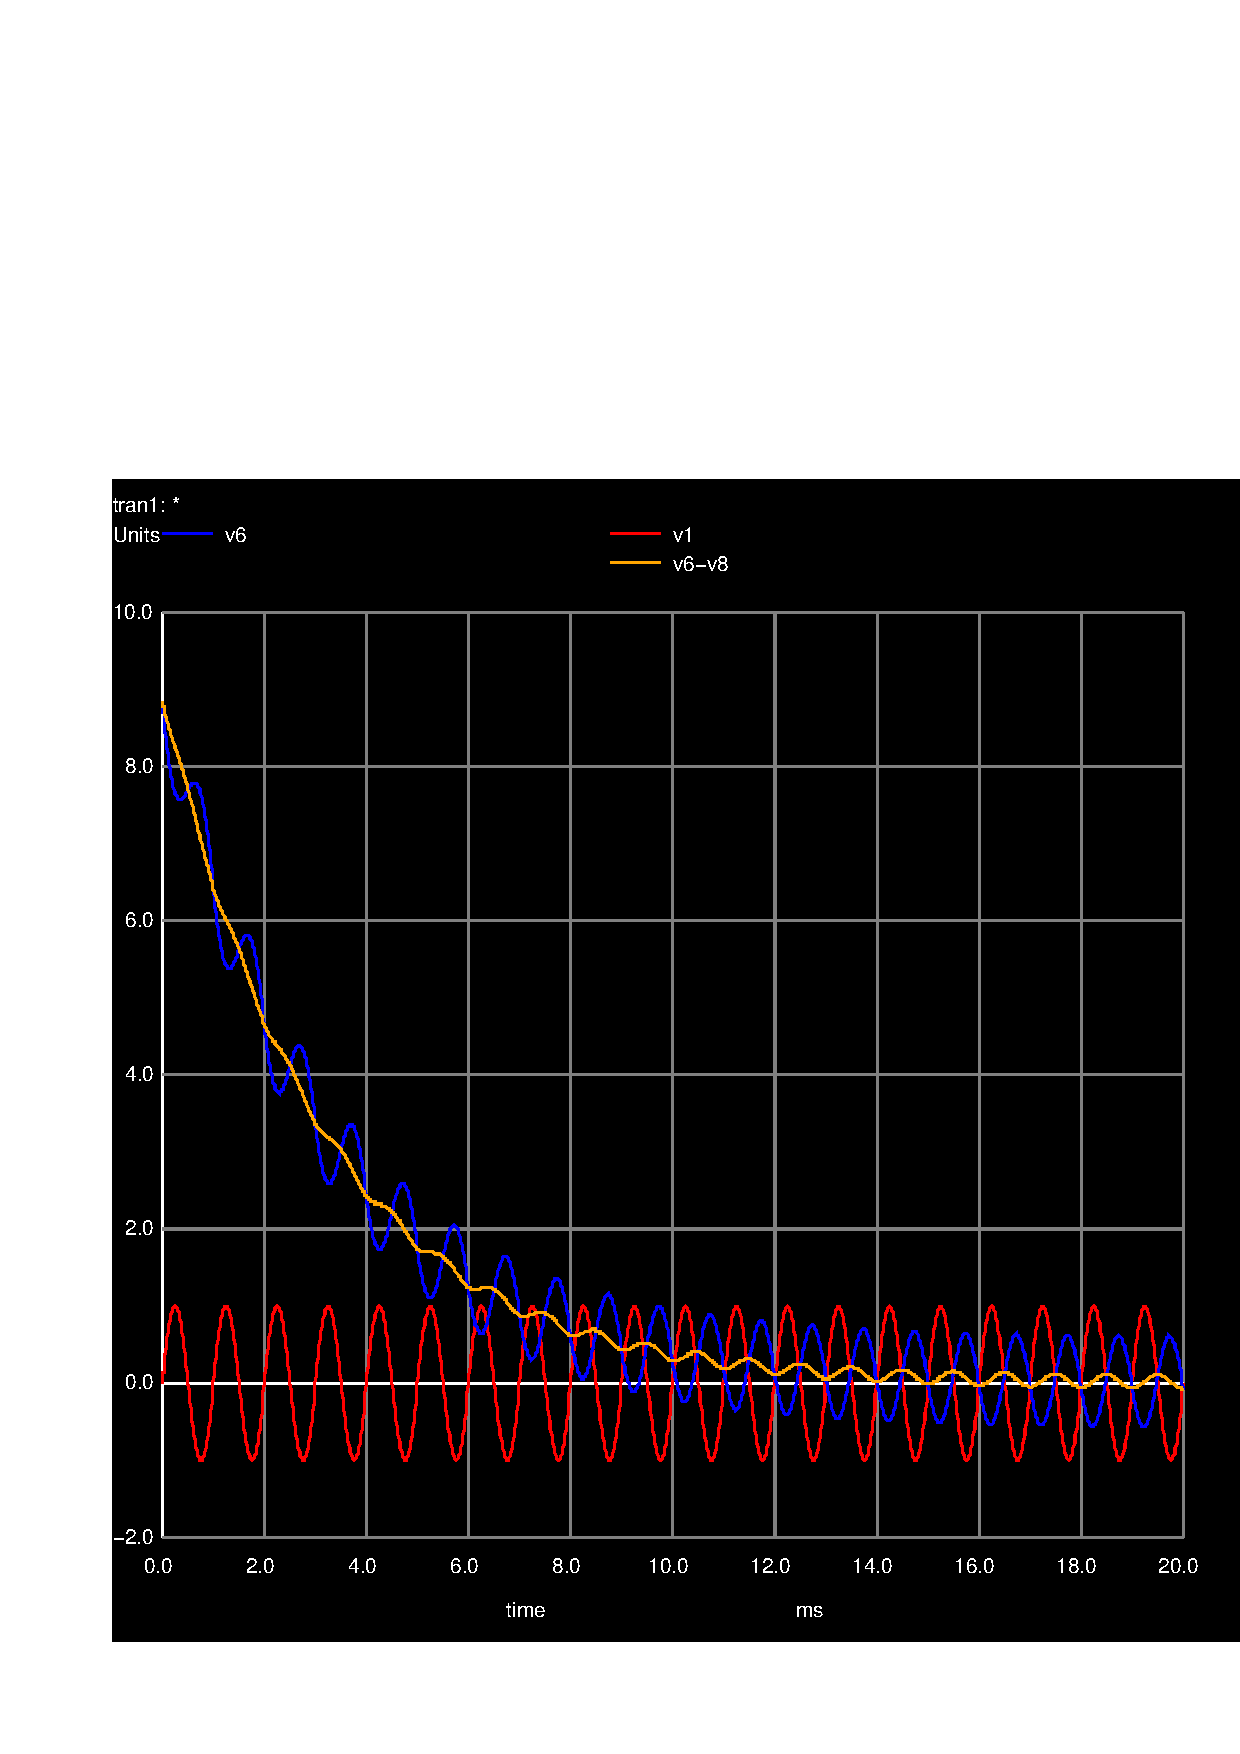
\includegraphics[width=0.4\linewidth]{trans2.pdf}
\caption{Transient input voltage of the secondary circuit and transient output voltage of both the envelope detector and 
voltage regulator and the average voltage difference.}
\label{fig:trans2}
\end{figure}

By analysing the result of the simulation we notice that the output solution resulted in an aproximated sinusoidal 
fuction: in fact, because of the average voltage is not ideal, the curve has an upward sinusoidal motion and 
a downward motion described by a negative exponential. The input voltage is described by a sinusoidal fuction, as expected. 
As far as the result is concerned, the form of the theoretical solution match the one obtained by NGSpice. 
Note that, because of the scale, we can not see the wave form of the ripple voltage and voltage difference because 
they are very small, which means that we obtained a decent result for 2 of the 3 parameters that influence the merit.


	Table~\ref{tab1:op} shows the measured results for the maximum, minimum and average output voltage of the circuit $V_4$. 
	Notice that the values on the right were obtained by Octave, therefore they are the theoretical values, which we already 
	mentioned previously but, to facilitate the comparison between the simulation and theoretical values, we mentioned them again.

\begin{table}[H]
  \centering
  \begin{tabular}{|l|r|}
    \hline    
    {\bf Name} & {\bf Voltage[V]} \\ \hline
    \input{../sim/op1_tab}
  \end{tabular}
  \begin{tabular}{|l|r|}
    \hline    
    {\bf Node} & {\bf Voltage[V]} \\ \hline
    \input{../mat/V_tab}
  \end{tabular}
  \caption {Measured maximum, minimum and average output voltage of the circuit. 
  The values on the right are the theoretical values for the same voltages in the circuit.}
  \label{tab1:op}
\end{table}


	Compared to the theoretical analysis results, we notice that both simulation results are accurate, except for the last 
decimal places, as a consequence of the cientific notation and the number of significative algharisms used by each program to 
present the results. Despite that, we realise that the values with more significant algharisms match correctly the rounded values.


Table~\ref{tab2:op} shows the ripple voltage of the circuit and the average voltage difference
between the output voltage and 12 Volts. Again, we show the theoretical values obtained for this step, 
to make it easier to compare between simulation and theoretical values.


\begin{table}[H]
  \centering
  \begin{tabular}{|l|r|}
    \hline    
    {\bf Name} & {\bf Voltage[V]} \\ \hline
    \input{../sim/op2_tab}
  \end{tabular}
  \begin{tabular}{|l|r|}
    \hline    
    {\bf Name} & {\bf Voltage[V]} \\ \hline
    \input{../mat/Ripple_tab}
  \end{tabular}
  \caption{Ripple voltage max$V_4$ - min$V_4$ and the average voltage difference $V_4$ - 12. The values on the right are the theoretical 
  values for the same voltages in the circuit.}
  \label{tab2:op}
\end{table}


Table~\ref{tab3:op} shows the total cost of the circuit and the figure of merit of the circuit. 
Note that we used the simulated voltage results to calculate the value of merit.


\begin{table}[H]
  \centering
  \begin{tabular}{|l|r|}
    \hline    
    {\bf Formula} & {\bf Merit} \\ \hline
    \input{../sim/op3_tab}
  \end{tabular}
  \caption{Figure of merit with a cost of 222.4 monetary units (MU).}
  \label{tab3:op}
\end{table}

By analising the figure of merit, we note that its value, considering the multiple results obtained for different values of the components and layots of the circuit, is
reasonable. Nevertheless, we consider the result not satisfying, since we obtained a merit of around 900 when we eliminated resistor $R_1$ and added 15 more diodes to the series
(reducing considerably the cost, the ripple and the average voltage difference). However, the AC/DC converter obtained would not be an efficient one, since it would have an enourmous
stabilization time and no resistor connected in parallel with the capacitor.

